\chapter{Лекция 5. Слабая и сильная связность. Граф Герца. Эйлеровость}

% === Слабая и сильная связность ===

Ориентированный граф $G(V, E)$.

% Граф: p11-example-6.graph (два примера в одном файле)
\grfig{figures/p11-example-6.pdf}{Изотропия/анизотропия}

\textbf{Пример} (изотропия): неориент. дерево $A$--$B$--$C$--$D$, $C$--$E$ ---
достижимость \textit{не зависит} от направления рёбер.

\textbf{Пример} (анизотропия): $A \to B \to C$ ---
достижимость \textit{зависит} от направления рёбер.

\begin{defn}{Слабая связность}{weak-connectivity}
$G(V, E)$ --- ориентированный граф.

$G$ --- \textbf{слабо связен} $\;\Leftrightarrow\;$ $G$ связен без учёта ориентации рёбер.
\end{defn}

\begin{defn}{Сильная связность}{strong-connectivity}
$G(V, E)$ --- ориентированный граф.

$G$ --- \textbf{сильно связен} $\;\Leftrightarrow\;$
$\forall\, u, v \in V$: $\exists$ путь $u \to \ldots \to v$.
\end{defn}

\begin{defn}{Компонента сильной связности}{scc}
\textbf{Компонента сильной связности} --- максимальный по включению
сильно связный подграф.
\end{defn}

\bigskip
% === Пример: ориент. граф и его SCC ===
% Граф: p12-example-1.graph (ориентированный)
\grfig{figures/p12-example-1.pdf}{Ориент. граф (SCC) + граф Герца}
% Вершины: A, B, C, D, E, F, H, I, J
% Рёбра: A→B, B→D, D→A, B→C, C→E, C→H, H→I, I→J, J→H, E→F, F→E

\textbf{Пример.} Ориентированный граф:
$A \to B$,\; $B \to D$,\; $D \to A$ (цикл);
$B \to C$;\;
$C \to E$,\; $E \to F$,\; $F \to E$ (цикл);\;
$C \to H$,\; $H \to I$,\; $I \to J$,\; $J \to H$ (цикл).

Компоненты сильной связности:
$\{A, B, D\}$,\quad $\{C\}$,\quad $\{E, F\}$,\quad $\{H, I, J\}$.

\bigskip
% === Граф Герца ===
\begin{defn}{Граф Герца (конденсации)}{hertz-graph}
$G(V, E)$ --- орграф.

\textbf{Граф Герца} (граф конденсации) для $G$ ---
$\tilde{G}(\tilde{V}, \tilde{E})$, где:
\begin{itemize}
  \item $\tilde{V} \ni w \;\Leftrightarrow\; w$ --- компонента сильной связности $G$;
  \item $\tilde{e} \in \tilde{E} \;\Leftrightarrow\;$ между соответствующими
        компонентами сильной связности в $G$ $\exists$ путь.
\end{itemize}
\end{defn}

\textbf{Граф Герца} для примера выше:

$\{A,B,D\} \to \{C\}$,\quad
$\{C\} \to \{E,F\}$,\quad
$\{C\} \to \{H,I,J\}$.

% Граф Герца также изображён в p12-example-1.graph (нижняя часть)

\medskip
\textbf{Тривиальные свойства графа Герца:}
\begin{enumerate}
  \item $\forall\, G$:\; $\tilde{G}$ существует и единственен;
  \item $\tilde{G}$ --- строго ориентированный;
  \item $\tilde{G}$ --- ациклический.
\end{enumerate}

\bigskip
% === Алгоритм Косарайю ===
\begin{algo}{Алгоритм Косарайю (построение графа Герца)}{kosaraju}
Алгоритм для выделения компонент сильной связности.

\medskip
\textbf{Шаг I.} Серия DFS: <<тупиковая>> вершина (все исходящие рёбра
которой уже обработаны) кладётся в стек. Стек заполняется снизу вверх
по порядку завершения обработки вершин.

\textit{Зачем это нужно:} если из компоненты $X$ есть путь в компоненту
$Y$ ($X$ <<выше по течению>>), то хотя бы одна вершина $X$ окажется в
стеке \emph{выше} всех вершин $Y$. Поэтому на шаге~III обход стартует
из компонент, <<выше по течению>>, и не <<перетекает>> в чужие компоненты.

\textbf{Шаг II.} $\operatorname{inv} E$ --- инвертируем все рёбра.

\textbf{Шаг III.} Серия DFS, согласованная со стеком: достаём вершины
с верха стека; из каждой ещё не помеченной вершины запускаем DFS по
\emph{инвертированным} рёбрам --- все достижимые непомеченные вершины
образуют одну компоненту сильной связности (красим своим цветом).

\textbf{Результат:} компоненты сильной связности; стянув каждую в одну
вершину, получаем граф Герца.

\medskip
\noindent\textbf{Работа алгоритма по шагам} (граф из примера выше;
стек показан справа, верх стека --- сверху):

\begin{center}\begin{tabular}{cc}
\shortstack{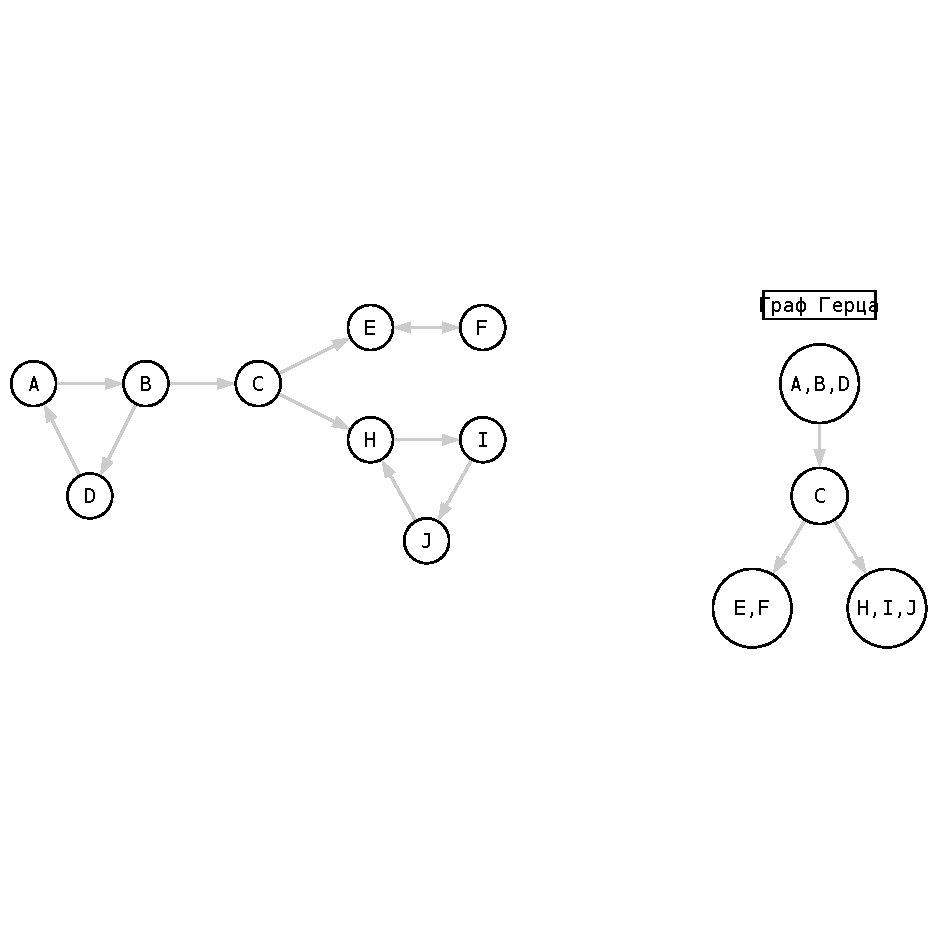
\includegraphics[width=0.46\textwidth]{python/lec05/kosaraju/kosaraju-0.pdf}\\[2pt]{\scriptsize Шаг 0. Исходный граф}} &
\shortstack{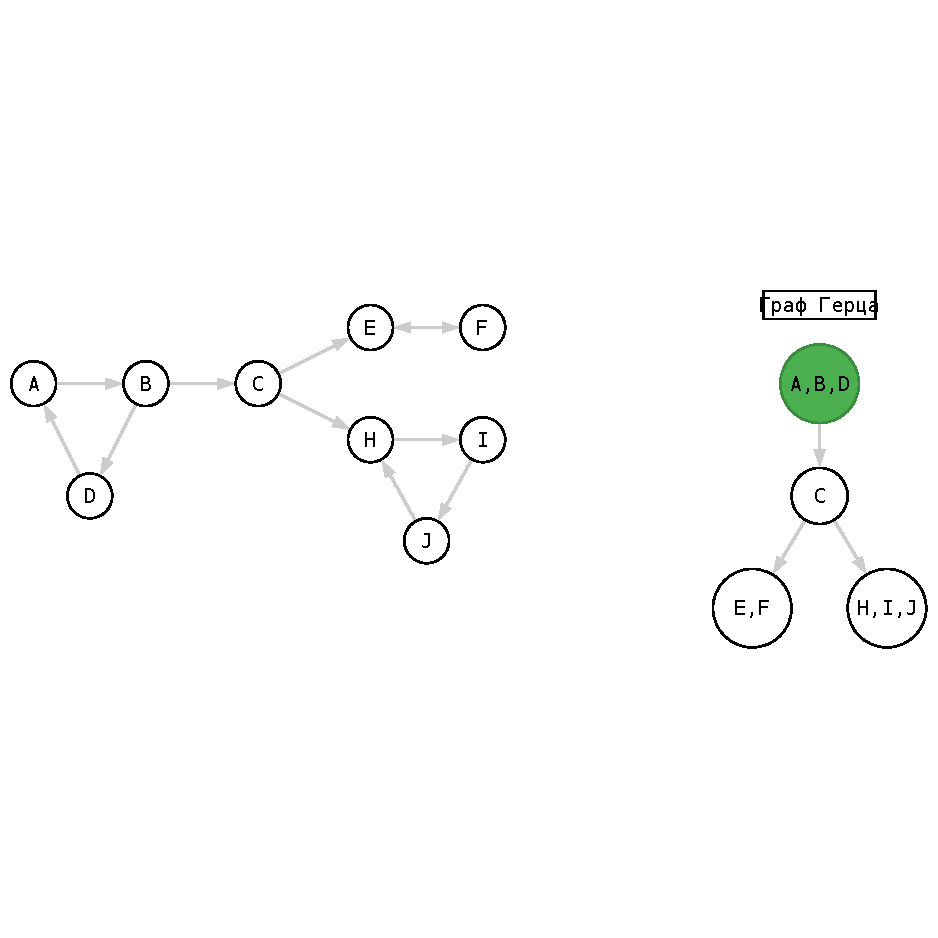
\includegraphics[width=0.46\textwidth]{python/lec05/kosaraju/kosaraju-1.pdf}\\[2pt]{\scriptsize Шаг 1. Серия DFS из $A$: стек по временам выхода}} \\
\end{tabular}\end{center}
\begin{center}\begin{tabular}{cc}
\shortstack{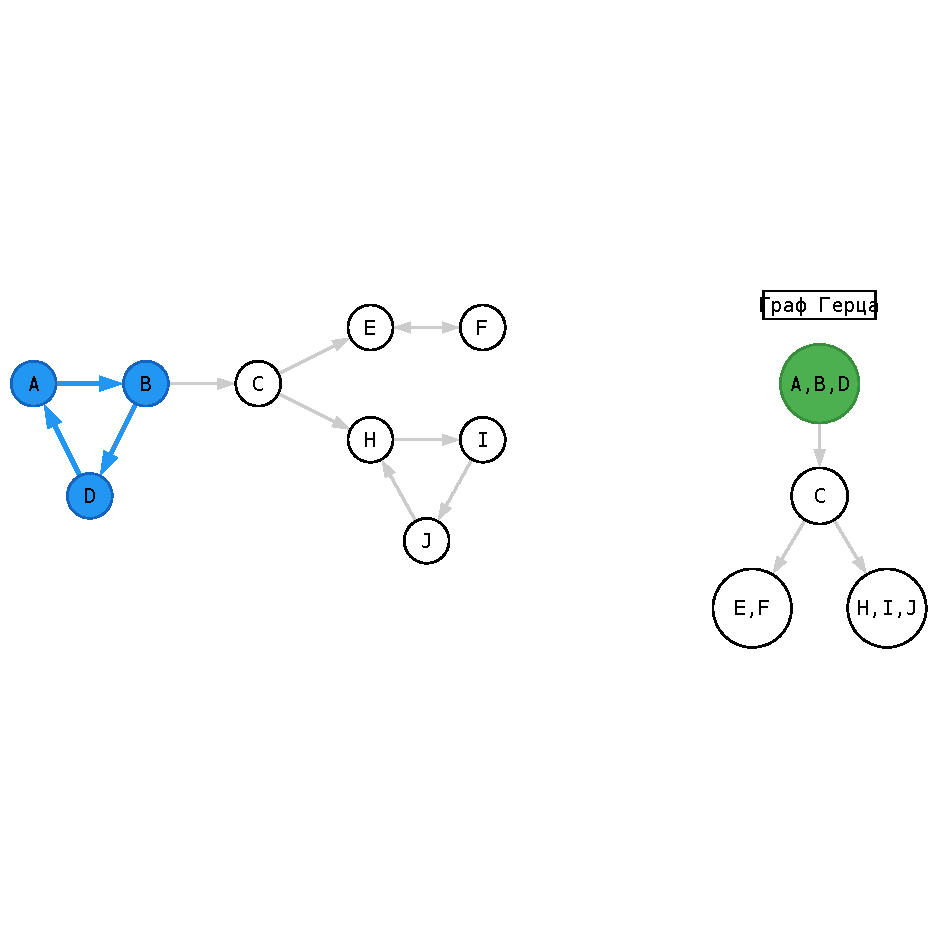
\includegraphics[width=0.46\textwidth]{python/lec05/kosaraju/kosaraju-2.pdf}\\[2pt]{\scriptsize Шаг 2. Инвертируем все рёбра}} &
\shortstack{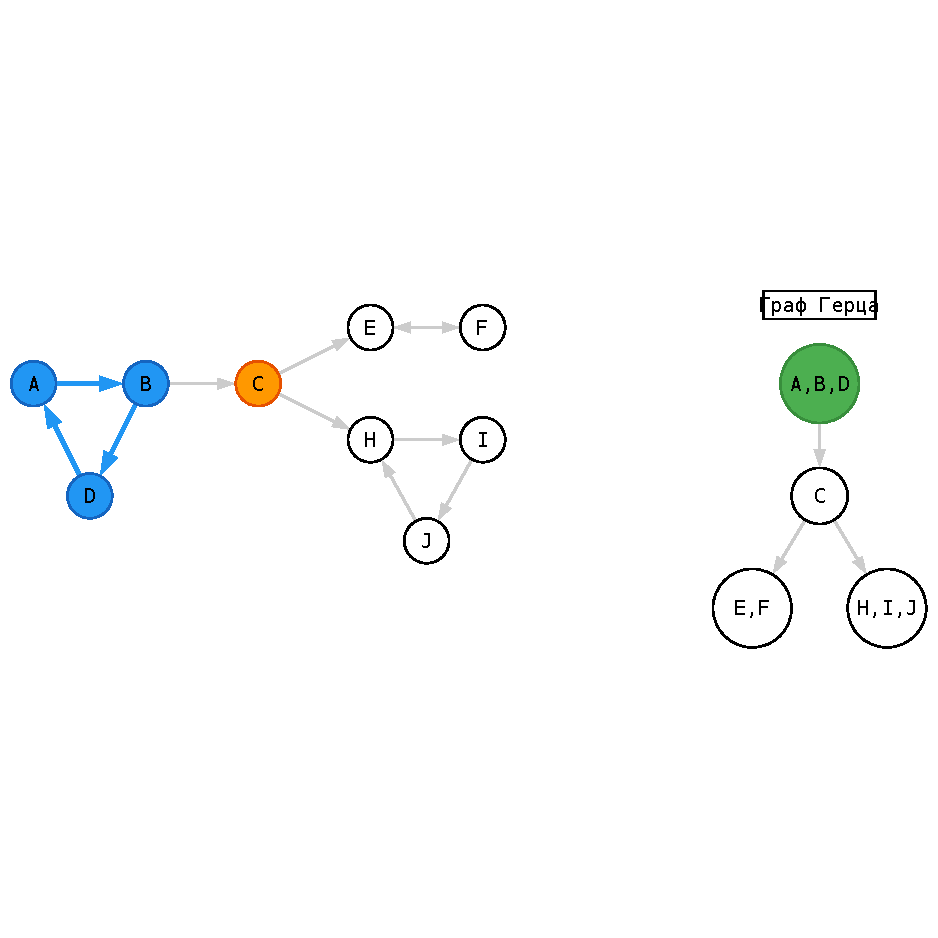
\includegraphics[width=0.46\textwidth]{python/lec05/kosaraju/kosaraju-3.pdf}\\[2pt]{\scriptsize Шаг 3. Сверху стека $A$: DFS даёт $\{A, D, B\}$}} \\
\end{tabular}\end{center}
\begin{center}\begin{tabular}{cc}
\shortstack{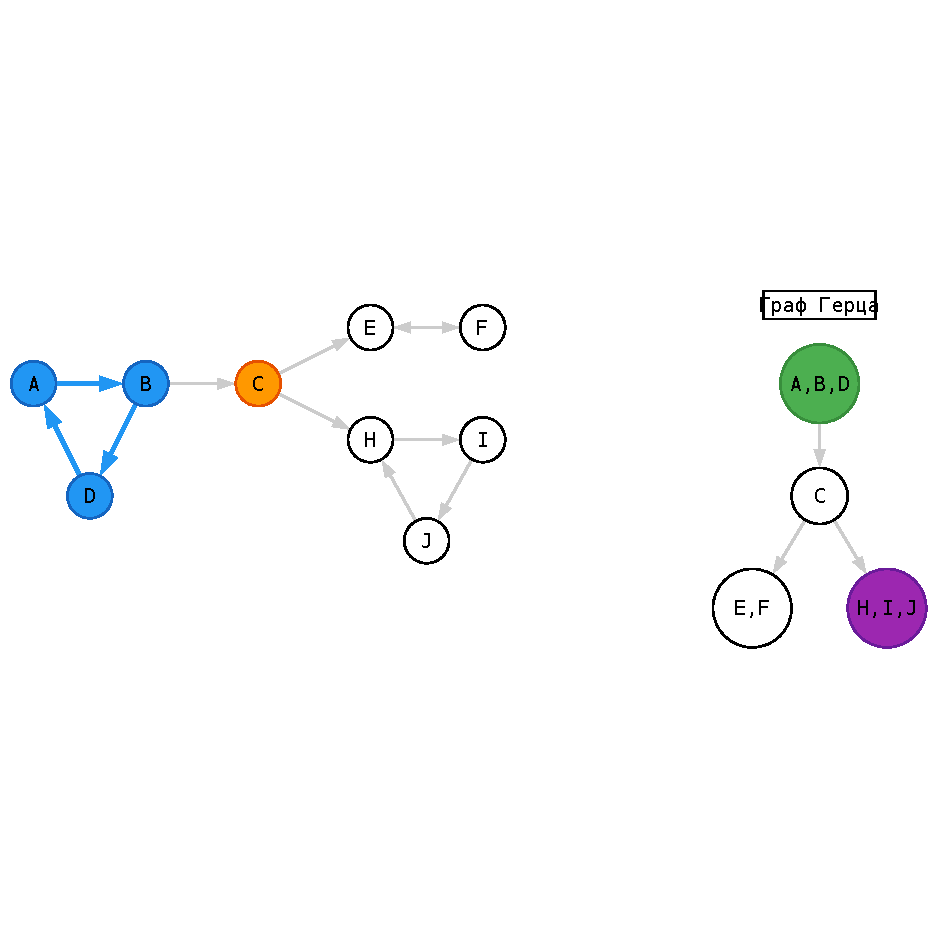
\includegraphics[width=0.46\textwidth]{python/lec05/kosaraju/kosaraju-4.pdf}\\[2pt]{\scriptsize Шаг 4. Следующая непомеченная $C$: $\{C\}$}} &
\shortstack{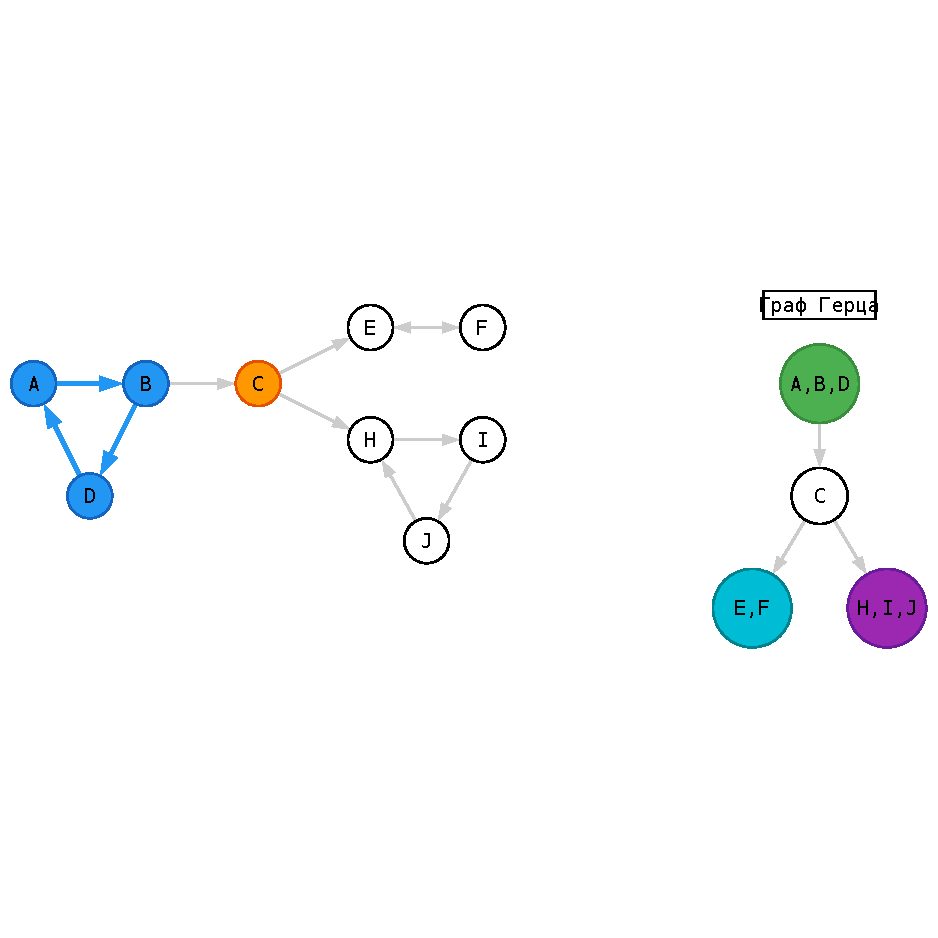
\includegraphics[width=0.46\textwidth]{python/lec05/kosaraju/kosaraju-5.pdf}\\[2pt]{\scriptsize Шаг 5. Из $H$: компонента $\{H, J, I\}$}} \\
\end{tabular}\end{center}
\begin{center}\begin{tabular}{cc}
\shortstack{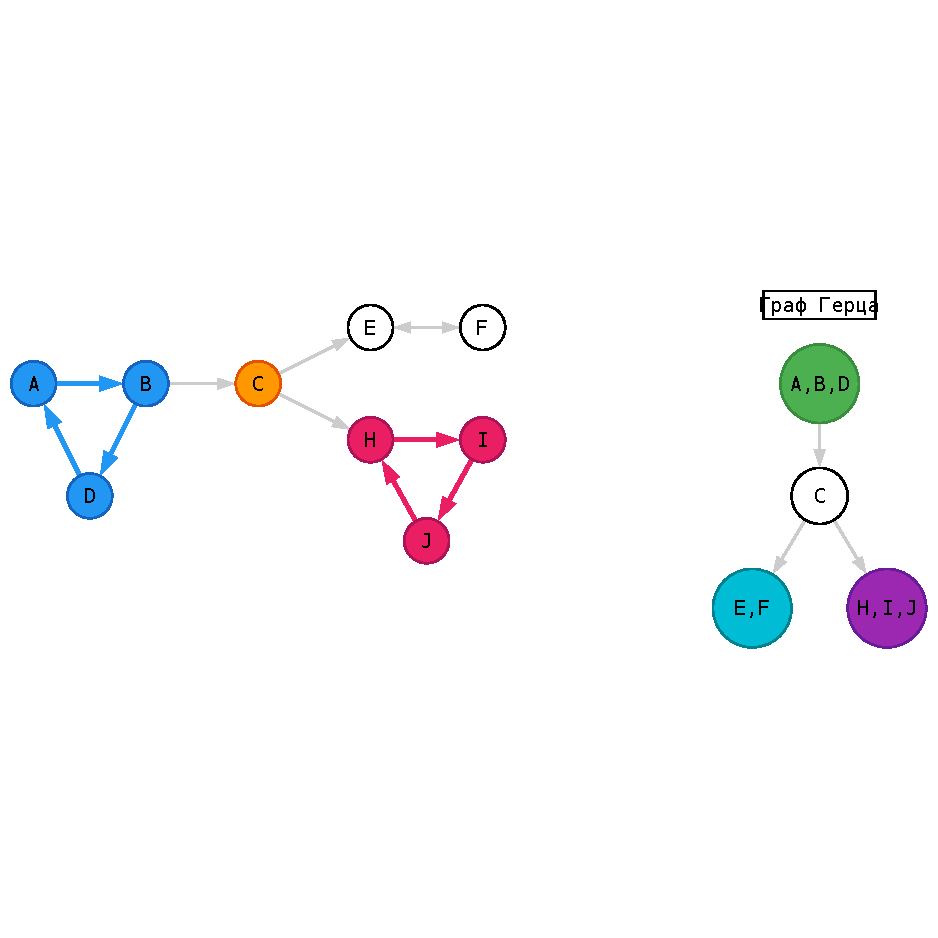
\includegraphics[width=0.46\textwidth]{python/lec05/kosaraju/kosaraju-6.pdf}\\[2pt]{\scriptsize Шаг 6. Из $E$: компонента $\{E, F\}$}} &
\shortstack{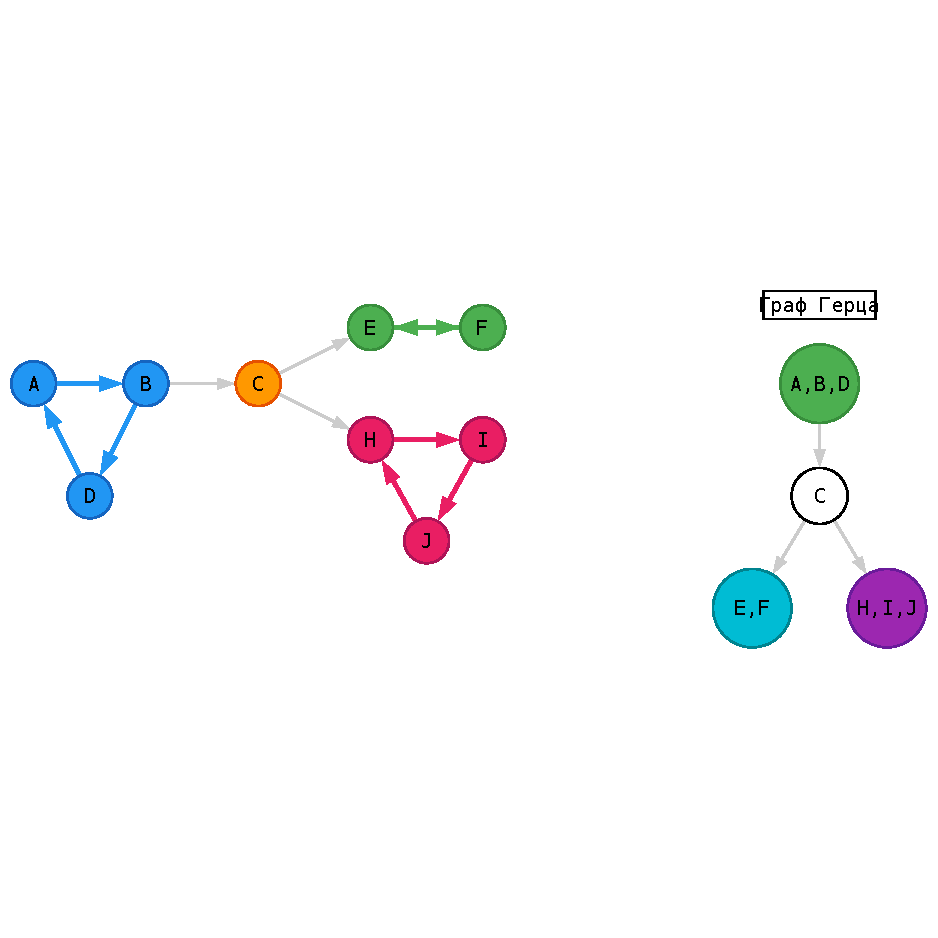
\includegraphics[width=0.46\textwidth]{python/lec05/kosaraju/kosaraju-7.pdf}\\[2pt]{\scriptsize Шаг 7. Итог: 4 компоненты сильной связности}} \\
\end{tabular}\end{center}

\noindent\textit{Комментарии к шагам.} На шаге~1 поиск в глубину из $A$
обходит граф: $A \to B \to D$ (ребро $D \to A$ ведёт в посещённую
вершину, $D$ --- тупиковая, кладём в стек); далее $B \to C \to E \to F$
(ребро $F \to E$ --- в посещённую, $F$ в стек, затем $E$);
$C \to H \to I \to J$ ($J \to H$ --- в посещённую, в стек уходят
$J$, $I$, $H$); наконец в стек уходят $C$, $B$, $A$. Стек снизу вверх:
$D, F, E, J, I, H, C, B, A$.

На шаге~III достаём вершины сверху: из $A$ по инвертированным рёбрам
достижимы $D$ и $B$ --- компонента $\{A, B, D\}$ (шаг~3); $B$ уже
помечена, следующая $C$ --- из неё по инвертированным рёбрам можно
попасть только в помеченную $B$, компонента $\{C\}$ (шаг~4); из $H$
достижимы $J$ и $I$ --- $\{H, I, J\}$ (шаг~5); из $E$ достижима $F$ ---
$\{E, F\}$ (шаг~6). Все вершины помечены --- алгоритм завершён (шаг~7).
\end{algo}

% ============================================================
% ЭЙЛЕРОВОСТЬ (стр. 13, dir2 стр. 1)
% ============================================================

\subsection*{Эйлеровость}

\begin{defn}{Эйлеров цикл и эйлеров путь}{euler}
Дан $G(V, E)$.

$G$ содержит \textbf{эйлеров цикл} $\;\Leftrightarrow\;$ $\exists$ в $G$ цикл, содержащий
$\forall\, e \in E$ ровно 1 раз.

$G$ содержит \textbf{эйлеров путь} $\;\Leftrightarrow\;$ в $G$ $\exists$ открытый простой
путь, содержащий $\forall\, e \in E$.
\end{defn}

\begin{defn}{Эйлеров граф}{euler-graph}
$G$ --- \textbf{эйлеров}:
\begin{itemize}
  \item $G$ --- ориент. $\;\Leftrightarrow\;$ в $G$ $\exists$ эйлеров цикл, $G$ --- слабо связен.
  \item $G$ --- неориент. $\;\Leftrightarrow\;$ в $G$ $\exists$ эйлеров цикл, $G$ --- связный.
\end{itemize}
\end{defn}

\begin{defn}{Полуэйлеров граф}{semi-euler-graph}
$G$ --- \textbf{полуэйлеров}:
\begin{itemize}
  \item $G$ --- ориент. $\;\Leftrightarrow\;$ в $G$ $\exists$ эйлеров путь, $G$ --- слабо связен.
  \item $G$ --- неориент. $\;\Leftrightarrow\;$ в $G$ $\exists$ эйлеров путь, $G$ --- связный.
\end{itemize}
\end{defn}

\medskip
\noindent\textbf{Примеры} (проверяем по степеням вершин):

% Пример 1: треугольник — Э
% Граф: p13-example-1.graph
\grfig{figures/p13-example-1.pdf}{Эйлеровость: пример 1 --- эйлеров}
\noindent\textit{Пример 1.} Цикл $1$--$2$--$3$--$1$: все степени равны $2$
(чётные), граф связный $\Rightarrow$ \textbf{эйлеров}; эйлеров цикл --- сам
треугольник.

% Пример 2: неориент. путь 1--2--3--4 — ПЭ
% Граф: p13-example-2.graph
\grfig{figures/p13-example-2.pdf}{Эйлеровость: пример 2 --- полуэйлеров}
\noindent\textit{Пример 2.} Цепь $1$--$2$--$3$--$4$: ровно две вершины
нечётной степени ($\deg 1 = \deg 4 = 1$), у остальных степень $2$
$\Rightarrow$ \textbf{полуэйлеров}; эйлеров путь --- сама цепь от $1$ до $4$.

% Пример 3: треугольник + два «уса» — ПЭ
% Граф: p13-example-3.graph
\grfig{figures/p13-example-3.pdf}{Эйлеровость: пример 3 --- полуэйлеров}
\noindent\textit{Пример 3.} Треугольник $1$--$2$--$3$ с <<усами>> $3$--$4$ и
$3$--$5$: нечётные степени ровно у двух вершин --- $\deg 4 = \deg 5 = 1$
(при этом $\deg 3 = 4$, $\deg 1 = \deg 2 = 2$) $\Rightarrow$
\textbf{полуэйлеров}; эйлеров путь, например, $4$--$3$--$1$--$2$--$3$--$5$.

% Пример 4: четыре вершины нечётной степени — ни Э, ни ПЭ
% Граф: p13-example-4.graph
\grfig{figures/p13-example-4.pdf}{Эйлеровость: пример 4 --- ни Э, ни ПЭ}
\noindent\textit{Пример 4.} Треугольник $1$--$2$--$3$ с <<усами>> $3$--$4$ и
$5$--$2$: нечётная степень у \emph{четырёх} вершин
($\deg 2 = \deg 3 = 3$, $\deg 4 = \deg 5 = 1$) $\Rightarrow$
\textbf{ни эйлеров, ни полуэйлеров}.

% Пример 5: все степени чётные — Э
% Граф: p13-example-5.graph
\grfig{figures/p13-example-5.pdf}{Эйлеровость: пример 5 --- эйлеров}
\noindent\textit{Пример 5.} Два цикла $1$--$2$--$3$--$1$ и
$2$--$4$--$5$--$2$ с общей вершиной $2$: все степени чётные
($\deg 2 = 4$, у остальных $2$), граф связный $\Rightarrow$
\textbf{эйлеров}; эйлеров цикл: $1$--$2$--$4$--$5$--$2$--$3$--$1$.

% Пример 6: K4 — ни Э, ни ПЭ
% Граф: p13-example-6.graph
\grfig{figures/p13-example-6.pdf}{Эйлеровость: пример 6 --- ни Э, ни ПЭ}
\noindent\textit{Пример 6.} Полный граф $K_4$: \emph{все четыре} вершины
имеют нечётную степень $3$ $\Rightarrow$ \textbf{ни эйлеров, ни
полуэйлеров}.

\begin{statement}{Критерий Э и ПЭ}{euler-criterion}

\textbf{I.} $G(V,E)$ --- неориент., связный.

\begin{enumerate}[label=\alph*)]
  \item $G$ --- Э $\;\Leftrightarrow\;$ $\forall\, v \in V$: $\deg(v) \vdots\; 2$
  \item $G$ --- ПЭ $\;\Leftrightarrow\;$ $\exists\, u \neq v \in V$: $\deg(u) \ndiv 2$,\; $\deg(v) \ndiv 2$, \\
        $\forall\, w \in V \setminus \{u, v\}$: $\deg(w) \vdots\; 2$
\end{enumerate}

\textbf{II.} $G$ --- ориент., связный (слабо).

\begin{enumerate}[label=\alph*)]
  \item $G$ --- Э $\;\Leftrightarrow\;$ $\forall\, v \in V$: $\delta^+(v) = \delta^-(v)$
  \item $G$ --- ПЭ $\;\Leftrightarrow\;$ $\exists\, u, v \in V$:
        $\delta^+(u) = \delta^-(u) + 1$,\;
        $\delta^-(v) = \delta^+(v) + 1$, \\
        $\forall\, w \in V \setminus \{u, v\}$: $\delta^+(w) = \delta^-(w)$
\end{enumerate}
\end{statement}

\begin{proof}[Доказательство (случай I)]
\textbf{a) Необходимость ($\Rightarrow$).} Пусть в $G$ есть эйлеров цикл.
Идя по циклу, мы в каждую вершину столько же раз <<входим>>, сколько
<<выходим>>, и каждое инцидентное вершине ребро используется ровно один
раз --- либо для входа, либо для выхода. Значит, рёбра при каждой вершине
разбиваются на пары <<вход--выход>>, и все степени чётны.

\textbf{a) Достаточность ($\Leftarrow$).} Пусть все степени чётны и $G$
связен; индукция по числу рёбер. Возьмём любую вершину $v_0$ и пойдём по
непройденным рёбрам, никогда не останавливаясь: войдя в вершину
$w \ne v_0$, мы заняли нечётное число её рёбер, а степень чётна --- значит,
есть свободное ребро для выхода. Застрять можно только в $v_0$, т.\,е.
получаем цикл $C$. Удалим рёбра $C$ из графа: степени снова чётны
(в каждой вершине цикл занял чётное число рёбер). Каждая компонента
оставшегося графа по предположению индукции имеет эйлеров цикл, причём
из связности $G$ каждая компонента пересекается с $C$ по вершине.
Вклеим эти циклы в $C$ при прохождении общих вершин --- получим эйлеров
цикл всего графа.

\textbf{b)} Сводится к пункту a): если ровно две вершины $u, v$ нечётны,
добавим фиктивное ребро $u$--$v$ --- все степени станут чётными, по
пункту a) существует эйлеров цикл; удалив из него фиктивное ребро,
получим эйлеров путь из $u$ в $v$. Обратно: эйлеров путь из $u$ в $v$
плюс фиктивное ребро $u$--$v$ дают эйлеров цикл, поэтому по пункту a)
все вершины, кроме $u$ и $v$, чётны, а $u$ и $v$ нечётны.

Случай II (ориентированный) доказывается дословно так же с заменой
степени на полустепени: внутри цикла в каждую вершину входим столько же
раз, сколько выходим, поэтому $\delta^+(v) = \delta^-(v)$, и наоборот.
\end{proof}

% ============================================================
% Алгоритм Флёри (стр. 14, dir2 стр. 2)
% ============================================================

\medskip
\textbf{Алгоритм поиска эйлерова пути / эйлерова цикла} (не единственные!).

\begin{algo}{Алгоритм Флёри}{fleury}
\textbf{Вход:} $G$ --- Э или ПЭ.

\textbf{Выход:} эйлеров цикл / эйлеров путь.

\medskip
\textbf{P.S.} Граф не может быть Э и ПЭ одновременно.

\medskip
\textbf{Инициализация:}
\begin{enumerate}
  \item Э $\;\Rightarrow\;$ $\operatorname{start} \in V$ --- любая вершина.
  \item ПЭ $\;\Rightarrow\;$ $\operatorname{start} \in V$: $\deg(v) \ndiv 2$.
  \item (ориент.) $\;\Rightarrow\;$ $\operatorname{start} \in V$: $\delta^-(v) = \delta^+(v) + 1$.
\end{enumerate}

\medskip
\textbf{Шаг (step):}
на каждом шаге идём по ребру, которое \textbf{не является мостом}
в оставшемся графе (если есть выбор). По мосту идём, только когда
другого ребра из текущей вершины нет. Пройденное ребро удаляем.

\medskip
\noindent\textbf{Пример.}
% Граф: p14-example-1.graph
\grfig[0.5]{figures/p14-example-1.pdf}{Алг. Флёри: пример графа}
Степени: $\deg A = \deg C = \deg E = 4$, $\deg B = \deg D = 3$ ---
ровно две нечётные вершины, граф полуэйлеров; стартуем из нечётной
вершины $B$ (закончим в $D$).

\medskip
\begin{center}
\begin{tabular}{c|c|c|l}
№ & вершина & ребро & комментарий (мосты в оставшемся графе) \\ \hline
1 & $B$ & $B$--$A$ & мостов нет, берём любое ребро \\
2 & $A$ & $A$--$C$ & мостов нет \\
3 & $C$ & $C$--$B$ & мостов нет \\
4 & $B$ & $B$--$E$ & единственное оставшееся ребро из $B$ \\
5 & $E$ & $E$--$C$ & $E$--$C$ не мост (цикл $C$--$D$--$E$ цел) \\
6 & $C$ & $C$--$D$ & единственное ребро из $C$ (мост, но выбора нет) \\
7 & $D$ & $D$--$E$ & $D$--$E$ не мост, а $D$--$A$ --- мост: избегаем \\
8 & $E$ & $E$--$A$ & единственное ребро из $E$ \\
9 & $A$ & $A$--$D$ & последнее ребро; финиш в $D$ \\
\end{tabular}
\end{center}

\medskip
Эйлеров путь: $B, A, C, B, E, C, D, E, A, D$ --- все $9$ рёбер ровно
по одному разу, от одной нечётной вершины ($B$) до другой ($D$).

\medskip
\noindent\textbf{Работа алгоритма по шагам} (номера на рёбрах ---
порядок прохождения; старт $B$ --- синий, текущая вершина --- оранжевая):

\begin{center}\begin{tabular}{cc}
\shortstack{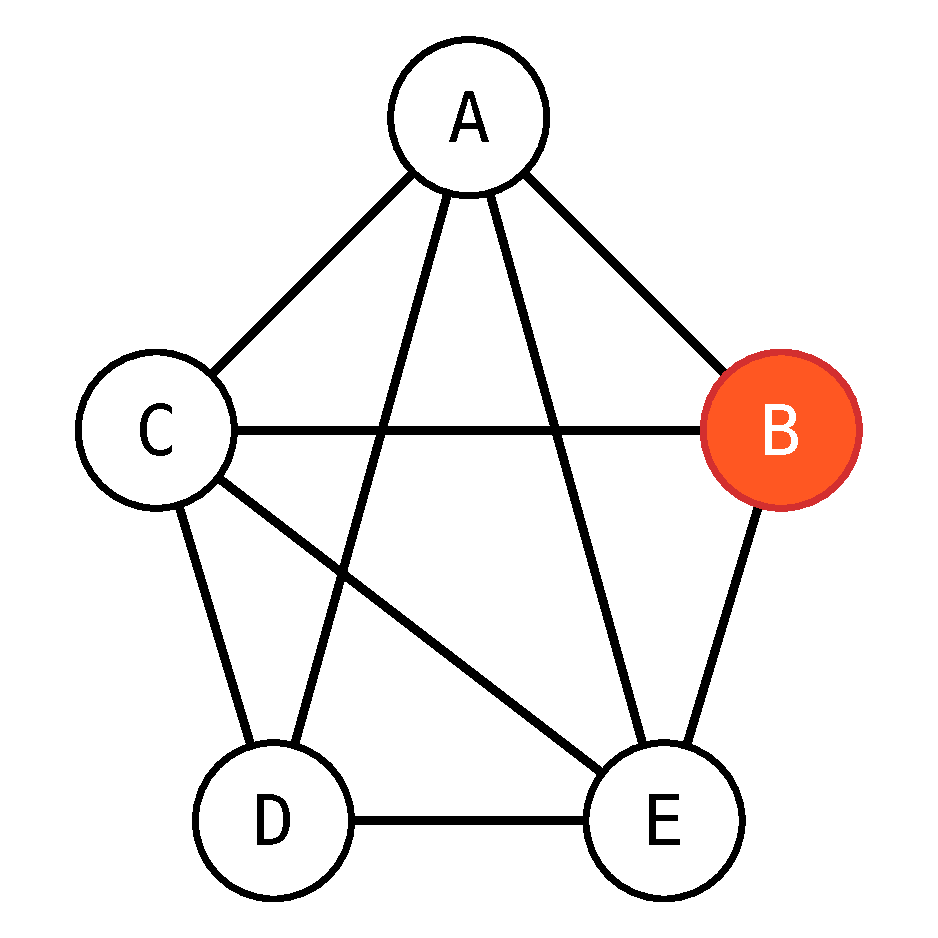
\includegraphics[width=0.40\textwidth]{python/lec05/fleury/fleury-0.pdf}\\[2pt]{\scriptsize Шаг 0. Старт в нечётной вершине $B$}} &
\shortstack{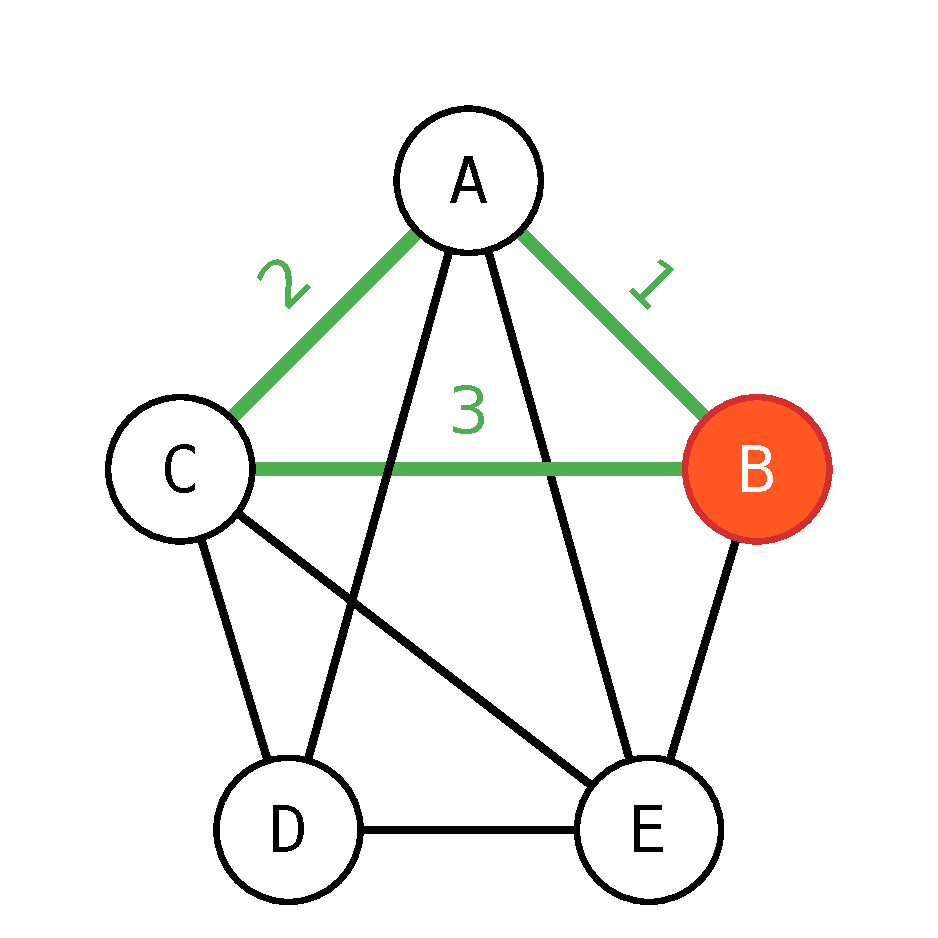
\includegraphics[width=0.40\textwidth]{python/lec05/fleury/fleury-1.pdf}\\[2pt]{\scriptsize Шаги 1--3: $B$--$A$--$C$--$B$}} \\
\end{tabular}\end{center}
\begin{center}\begin{tabular}{cc}
\shortstack{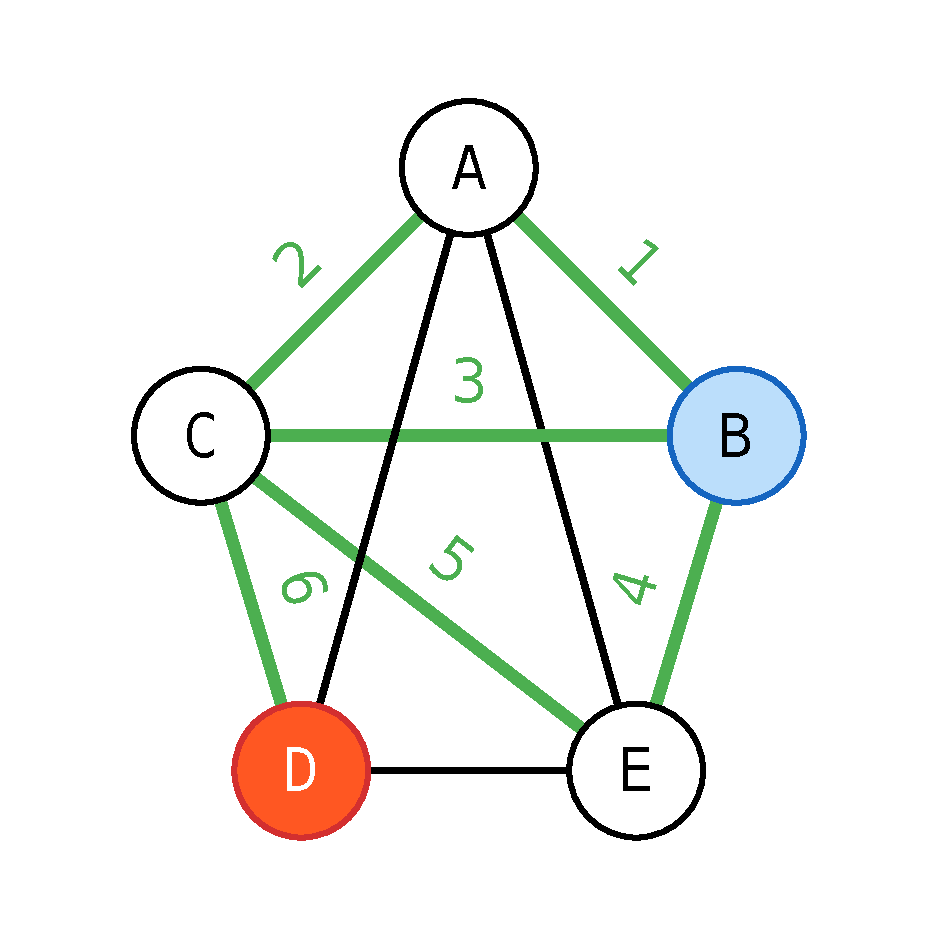
\includegraphics[width=0.40\textwidth]{python/lec05/fleury/fleury-2.pdf}\\[2pt]{\scriptsize Шаги 4--6: $B$--$E$--$C$--$D$}} &
\shortstack{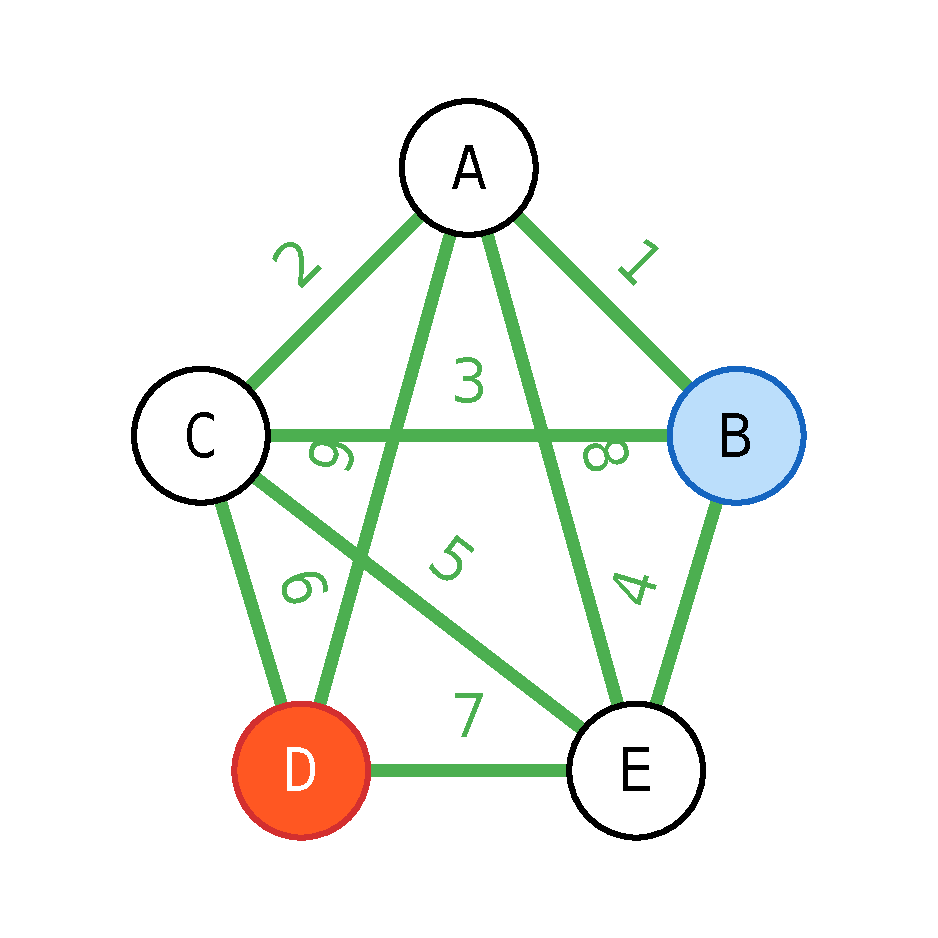
\includegraphics[width=0.40\textwidth]{python/lec05/fleury/fleury-3.pdf}\\[2pt]{\scriptsize Шаги 7--9: $D$--$E$--$A$--$D$, финиш в $D$}} \\
\end{tabular}\end{center}
\end{algo}

% ============================================================
% Алгоритм (на списках инцидентности) — стр. 14
% ============================================================

\begin{algo}{Алгоритм поиска эйлерова цикла (на списках инцидентности)}{euler-incidence}
\textbf{Идея.} Граф задан списками инцидентности (для каждой вершины ---
список исходящих рёбер). Используются стек \texttt{temp} и список
\texttt{result}:

\begin{enumerate}
  \item кладём стартовую вершину в стек;
  \item пока стек не пуст, смотрим на вершину $v$ с верха стека:
  \begin{itemize}
    \item если в списке $v$ осталось неиспользованное ребро $v \to u$ ---
          вычёркиваем его из списка и кладём $u$ в стек;
    \item если список $v$ исчерпан --- снимаем $v$ со стека и дописываем
          её в \texttt{result};
  \end{itemize}
  \item в конце \texttt{result}, прочитанный \emph{в обратном порядке},
        --- эйлеров цикл (путь).
\end{enumerate}

\medskip
\noindent\textbf{Пример.}
% Граф: p14-example-2.graph
\grfig[0.5]{figures/p14-example-2.pdf}{Алг. на списках инцидентности}
% Дуги: A→B, B→C, D→C, A→D, E→D, K→E, D→K, C→A, C→E, E→C

Полустепени: у вершины $A$ выходов на один больше, чем входов
($\delta^- (A) = 2$, $\delta^+(A) = 1$), у $C$ --- наоборот
($\delta^-(C) = 2$, $\delta^+(C) = 3$), у остальных входы равны выходам
--- по критерию граф полуэйлеров; эйлеров путь идёт из $A$ в $C$.

\medskip
\noindent Списки инцидентности (исходящие рёбра):

\begin{center}
\begin{tabular}{ll}
$A$: & $B,\; D$ \\
$B$: & $C$ \\
$C$: & $A,\; E$ \\
$D$: & $C,\; K$ \\
$E$: & $D,\; C$ \\
$K$: & $E$ \\
\end{tabular}
\end{center}

\medskip
\noindent Работа алгоритма: сначала стек только растёт ---
$A \to B \to C \to A \to D \to C \to E \to D \to K \to E \to C$ (каждый
раз вычёркиваем первое неиспользованное ребро из списка текущей вершины).
К этому моменту все $10$ рёбер израсходованы, и стек начинает
разбираться: вершины по очереди исчерпаны и уходят в \texttt{result}.

\medskip
\noindent Состояния (\texttt{temp} --- стек после фазы роста, читается
снизу вверх; \texttt{result} --- порядок выгрузки, сверху вниз):

\medskip
\begin{center}
\begin{tabular}{c|c}
\textbf{temp} (низ $\to$ верх) & \textbf{result} \\ \hline
$A$ & $C$ \\
$B$ & $E$ \\
$C$ & $K$ \\
$A$ & $D$ \\
$D$ & $E$ \\
$C$ & $C$ \\
$E$ & $D$ \\
$D$ & $A$ \\
$K$ & $C$ \\
$E$ & $B$ \\
$C$ & $A$ \\
\end{tabular}
\end{center}

\medskip
Эйлеров путь --- это \texttt{result}, прочитанный снизу вверх:
\[
  A,\; B,\; C,\; A,\; D,\; C,\; E,\; D,\; K,\; E,\; C
\]
--- все $10$ дуг ровно по одному разу, из $A$ в $C$.
\end{algo}

% ============================================================
\begin{task}{Эйлеровость графа}{euler-task}
\textbf{Условие.} Дан связный граф на вершинах $A,B,C,D$ с рёбрами
$AB,\ BC,\ CD,\ DA,\ AC$. Выясните, является ли он эйлеровым или
полуэйлеровым, и при возможности укажите эйлеров путь/цикл.

\begin{center}
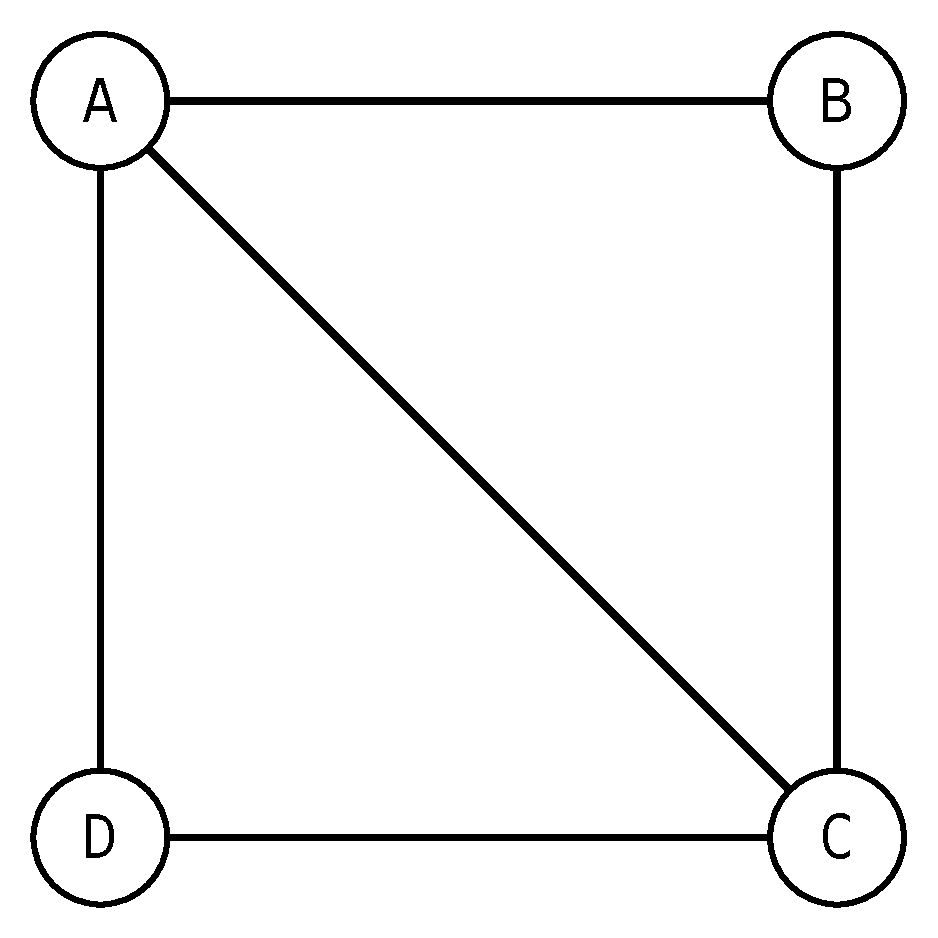
\includegraphics[width=0.32\textwidth]{figures/task-euler-1.pdf}
\end{center}

\smallskip
\textbf{Решение.} Применим критерий Эйлера: связный граф эйлеров (есть эйлеров
цикл) $\Leftrightarrow$ все степени вершин чётны; полуэйлеров (есть эйлеров
путь, но не цикл) $\Leftrightarrow$ ровно две вершины нечётной степени.

Подсчитаем степени:
\[
  \deg A=3\ (B,D,C),\quad \deg B=2\ (A,C),\quad \deg C=3\ (B,D,A),\quad \deg D=2\ (C,A).
\]
Нечётную степень имеют ровно две вершины --- $A$ и $C$. Следовательно, граф
\emph{полуэйлеров}: эйлерова цикла нет, но есть эйлеров путь, причём он обязан
начинаться и заканчиваться в нечётных вершинах $A$ и $C$.

Построим путь (например, алгоритмом Флёри, не выбирая мост, пока есть
альтернатива): 
\[
  A \to B \to C \to D \to A \to C.
\]
Он проходит по всем пяти рёбрам $AB,BC,CD,DA,AC$ ровно по одному разу
(номера на рёбрах --- порядок прохождения):

\begin{center}
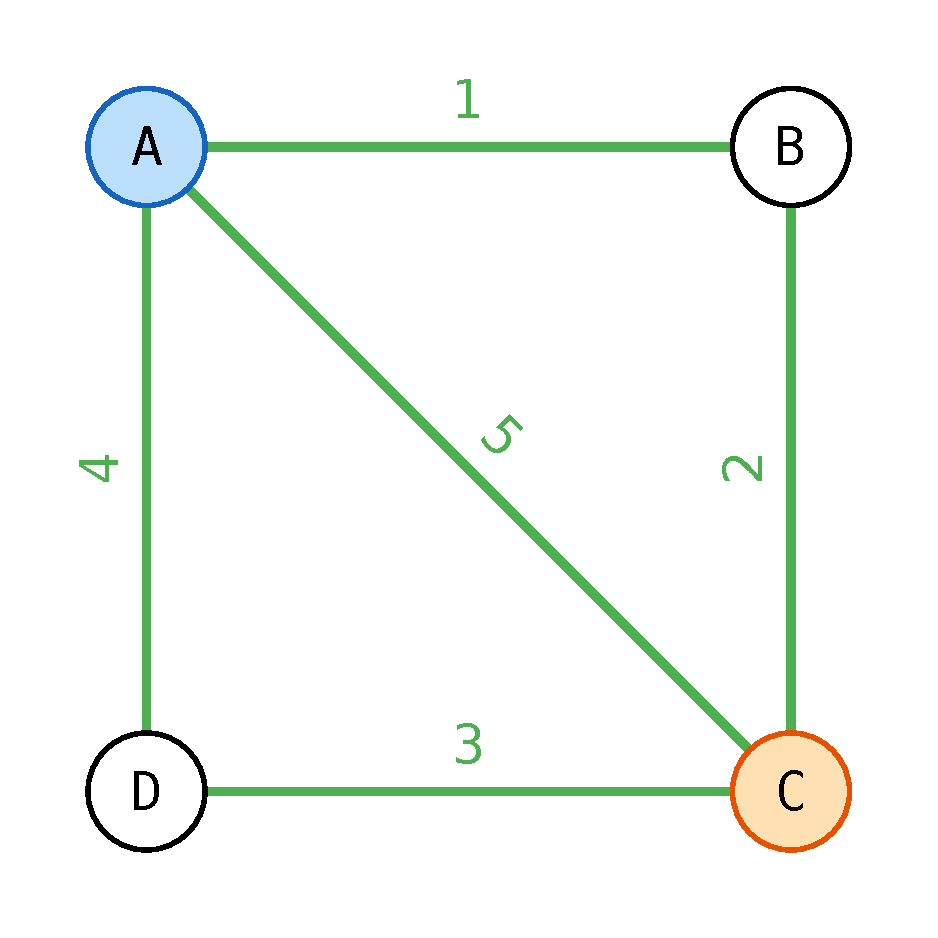
\includegraphics[width=0.32\textwidth]{figures/task-euler-2.pdf}
\end{center}

\textbf{Ответ.} Граф полуэйлеров; эйлеров путь $A\!-\!B\!-\!C\!-\!D\!-\!A\!-\!C$
(из $A$ в $C$). Эйлерова цикла нет, так как есть вершины нечётной степени.
\end{task}

% ============================================================
\begin{task}{Компоненты сильной связности: алгоритм Косарайю}{kosaraju-task}
\textbf{Условие.} Дан ориентированный граф на вершинах $A,B,C,D,E$ с дугами
\[
  A\!\to\!B,\ B\!\to\!C,\ C\!\to\!A,\ B\!\to\!D,\ D\!\to\!E,\ E\!\to\!D.
\]
Найдите компоненты сильной связности алгоритмом Косарайю.

\begin{center}
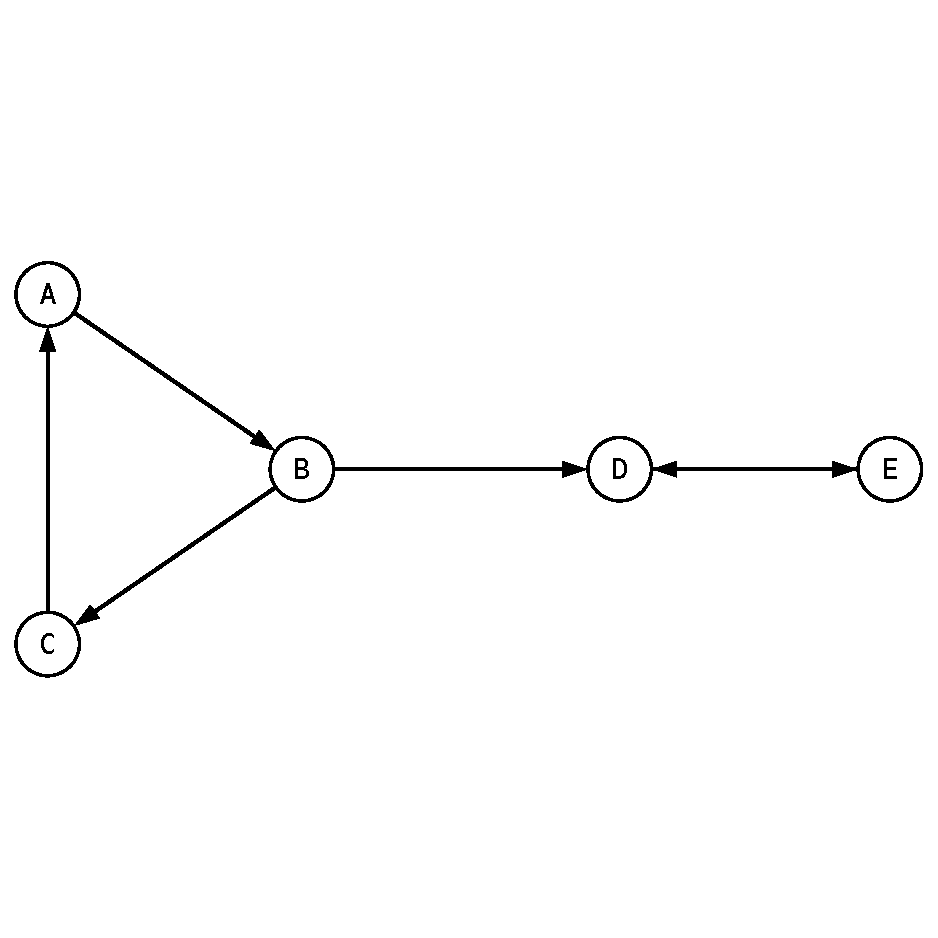
\includegraphics[width=0.45\textwidth]{figures/task-scc-1.pdf}
\end{center}

\smallskip
\textbf{Решение.} Алгоритм Косарайю состоит из трёх шагов: (1)~обход в глубину
исходного графа $G$ с записью времён выхода; (2)~построение транспонированного
графа $G^{T}$ (все дуги развёрнуты); (3)~обход $G^{T}$ в порядке убывания времён
выхода --- каждое дерево обхода даёт одну компоненту.

\textbf{Шаг 1. DFS по $G$ из $A$.} Порядок выхода (по возрастанию):
\[
  C(1),\ E(2),\ D(3),\ B(4),\ A(5).
\]
Порядок убывания времён выхода: $A,\ B,\ D,\ E,\ C$.

\textbf{Шаг 2. Транспонированный граф $G^{T}$:}
\[
  B\!\to\!A,\ C\!\to\!B,\ A\!\to\!C,\ D\!\to\!B,\ E\!\to\!D,\ D\!\to\!E.
\]

\textbf{Шаг 3. DFS по $G^{T}$ в порядке $A,B,D,E,C$.}
\begin{itemize}
  \item Из $A$: $A\!\to\!C\!\to\!B\!\to\!A$ --- собрана компонента $\{A,B,C\}$.
  \item Следующая непосещённая (по порядку) --- $D$: $D\!\to\!E\!\to\!D$ ---
        компонента $\{D,E\}$.
\end{itemize}

\begin{center}
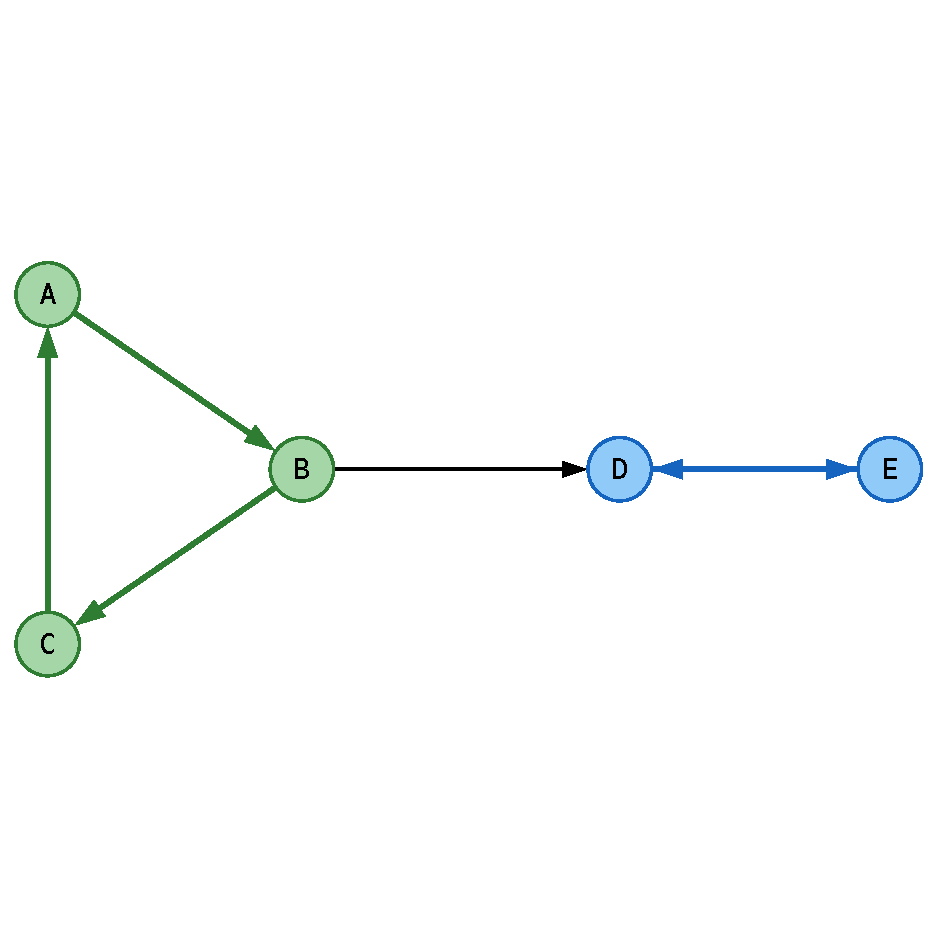
\includegraphics[width=0.45\textwidth]{figures/task-scc-2.pdf}
\end{center}

\textbf{Ответ.} Две компоненты сильной связности: $\{A,B,C\}$ (цикл
$A\!\to\!B\!\to\!C\!\to\!A$) и $\{D,E\}$ (цикл $D\!\leftrightarrows\!E$). Дуга
$B\!\to\!D$ соединяет компоненты в одном направлении, поэтому в одну компоненту
они не объединяются.
\end{task}
